\documentclass[12pt,a4paper]{article}
\usepackage[utf8]{inputenc}
\usepackage{amsmath}
\usepackage{amsfonts}
\usepackage{amssymb}
\usepackage{graphicx}
\usepackage[left=2cm,right=2cm,top=2cm,bottom=2cm]{geometry}
\usepackage[unicode]{hyperref}
\usepackage{tabularx} 

\setlength{\parindent}{0pt}
\setlength{\parskip}{0.35em}

\title{\textbf{Finding a Good Location to Open Thailand Restaurant in Jakarta, Indonesia.}\\{\normalsize \textit{A final report for the course ``Applied Data Science Capstone" given by IBM on Coursera}}}
\author{\textbf{imamjabar}}
\renewcommand{\today}{\ifcase \month \or January\or February\or March\or %
April\or May \or June\or July\or August\or September\or October\or November\or %
December\fi, \number \year} 

\usepackage[
    backend=biber,
    style=numeric,
    natbib=true,
    url=true, 
    doi=true,
    eprint=false
]{biblatex}

\addbibresource{myref.bib}

\begin{document}

\maketitle

\tableofcontents

\section{Problem's description}
\label{sec:problem}

The city of Jakarta is well known to be a cosmopolitan city where you can find people from all around the world with over 11 million people live and it has a population density of over 16 thousand people per square kilometer. The city is divided into 44 districts in total (including Thousand Island districts).

An investor is looking to open a new \textbf{Thailand Restaurant} in Jakarta, but he is not sure about the best location for his new venue and needs input for making the decision. Although there are a lot of districts in Jakarta, their density between them is not uniform. Some districts are containing too many restaurants while there are less in some others.

If we have some knowledge about the population density, the housing price in each district coupling with an overview of the number of restaurants, we can have a better idea to set up a new business there. We expect to choose a place where the population density is high but fewer competitors. If the housing price in that place is low, it’s more attractive to us.

The project aims to find a good location for a Thailand Restaurant in Jakarta. This will be determined by analyzing the number of restaurants, the population density, and the average housing price in each district.

\section{Data Description}

\begin{enumerate}
\item List of Jakarta City administrative units from \textbf{official Jakarta annual publication} and \textbf{OpenStreetMap mapping project}. It gives us a list of all urban districts of Jakarta with their area (in km$^2$), population (in 2020), and the density of each district (people/km$^2$). The list is given in \url{https://bit.ly/32NpEPQ}.
\item List of the coordinates (latitude, longitude) of 42 urban districts in Jakarta (without Seribu Island). This list can be generated based on the name of each district using \textbf{Nominatim} package. \textit{geopy.geocoders.Nominatim}.
\item List of average housing prices per m² from \textbf{real estate marketplace web page} \url{https://www.lamudi.co.id/trends/}.
\item A modified \textit{.json} file that contains all coordinates where we use it to create a choropleth map of the Housing Sales Price Index of Jakarta. From \textbf{Jakarta Geospatial Information site} \url{http://gis.bpbd.jakarta.go.id/layers/geonode%3Adki_kecamatan}.
\item \textbf{Foursquare API} to select the number of restaurants and their location in some neighborhoods of Jakarta \url{https://developer.foursquare.com/}.
\end{enumerate}

\section{Methodology}
\label{sec:method}

\begin{enumerate}
\item First, we need to collect all urban districts of Jakarta data from Jakarta annual publication to get \textbf{District Name}, \textbf{Area}, and \textbf{Population}. Also, collect \textbf{Average Housing Price} from the real estate marketplace. Then save it to \textit{.csv} file.
\item The column \textbf{Density} is calculated later based on columns \textbf{Population} and \textbf{Area} of each district.
\item Throughout the project, we use \textbf{numpy} and \textbf{pandas} packages to manipulate data frames
\item We use \textit{geopy.geocoders.Nominatim} package to get the coordinates of districts and add them to the main data frame.
\item We use \textbf{Foursquare API} to explore Thailand Restaurant venues in each district.
\item For clustering the "Thailand Restaurant" venues between districts, we use \textbf{K-Means Clustering} method and the package \textbf{scikit-learn} to implement the algorithm on our data. In order to indicate how many K for the method, we try with 10 different values of K from 1 to 10 and use the \textbf{elbow method} to choose the most appropriate one.
\item In order to visualize the charts, we use package \textbf{matplotlib} and \textbf{seaborn}.
\item We use the package \textbf{folium} to visualize the Jakarta map with its districts.
\end{enumerate}

\subsection{Data Preparation}
I read the data that I collected from the Jakarta annual report and real estate marketplace that I store in GitHub repository, which contains \textit{City name}, \textit{District}, \textit{Area}, \textit{Population}, and \textit{Average Housing Price}. Then I calculate the \textit{Density} based on columns population and area of each district. I use Nominator to get the \textit{Latitude} and \textit{Longitude} of all districts.

\begin{center}
    \begin{figure}[htp]
    \begin{center}
     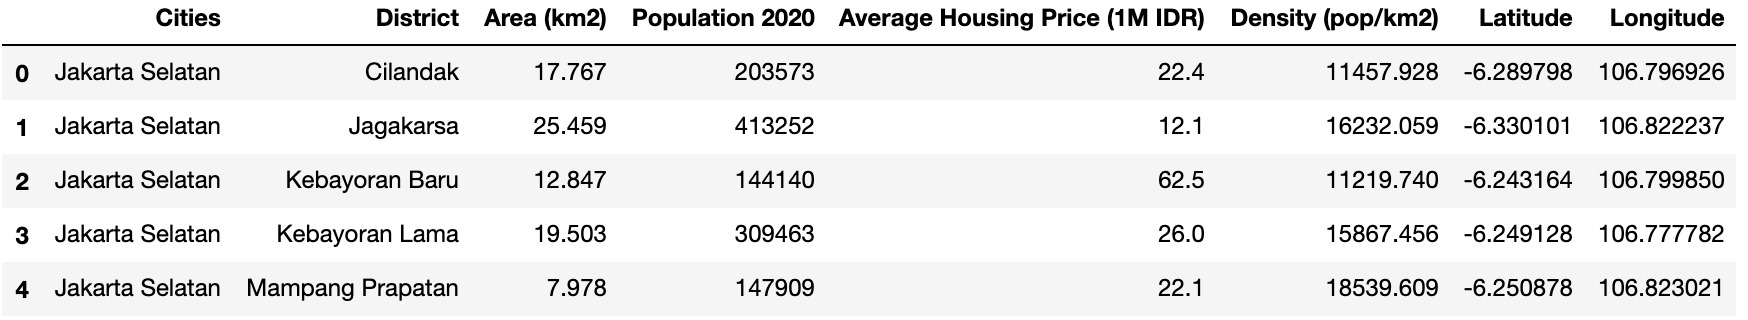
\includegraphics[width=\textwidth]{fig/df}
    \end{center}
    \caption{The main data frame.}
    \label{fig:df}
    \end{figure}
\end{center}

I used python Folium library to visualize geographic details of Jakarta and its districts and I created a map of Jakarta with districts superimposed on top. I used latitude and longitude values to get the visual as below:

\begin{center}
    \begin{figure}[htp]
    \begin{center}
     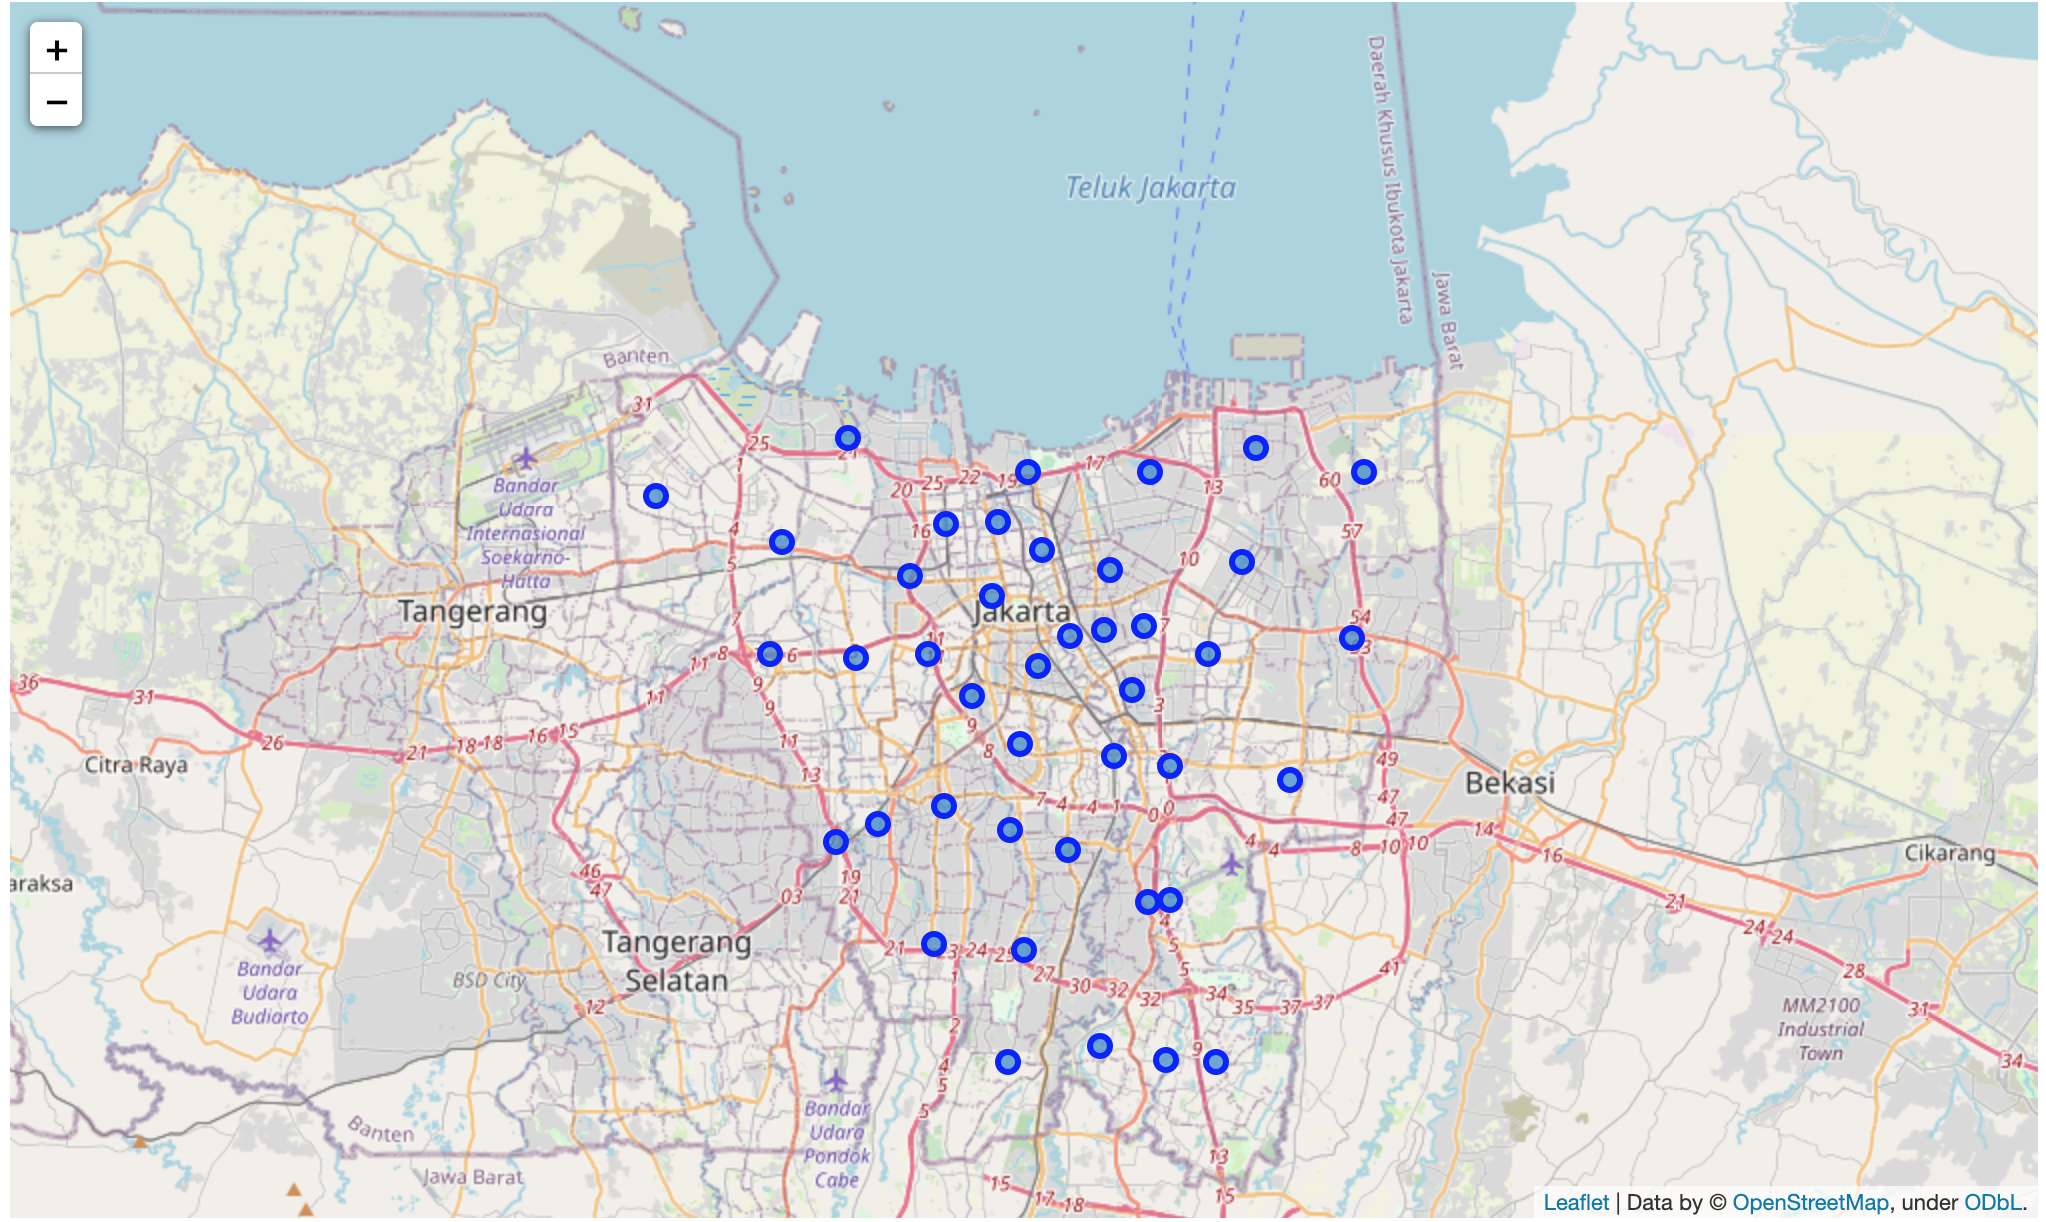
\includegraphics[width=0.8\textwidth]{fig/jakarta}
    \end{center}
    \caption{District of Jakarta}
    \label{fig:jakarta}
    \end{figure}
\end{center}

I utilized the Foursquare API to explore all \textbf{Thai Restaurants} venues in each District using the category parameter of Thai Restaurant from Foursquare. I designed the limit as 100 venue and the radius 5000 meter for each district from their given latitude and longitude information, and . Here is a head of the list \textit{id}, \textit{Venues name}, \textit{latitude and longitude}, \textit{distance} and \textit{category} from Foursquare API.

\begin{center}
    \begin{figure}[htp]
    \begin{center}
     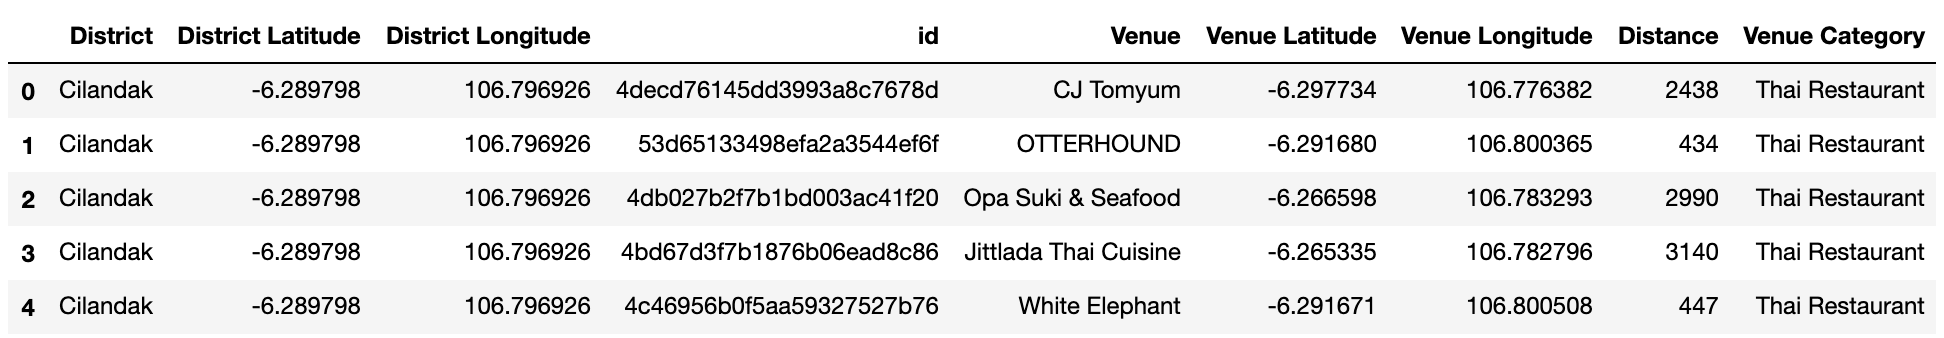
\includegraphics[width=0.7\textwidth]{fig/venues}
    \end{center}
    \caption{List of Venues}
    \label{fig:venues}
    \end{figure}
\end{center}

\clearpage

2021 venues were returned by Foursquare, but the data contain other venues than Thai Restaurant categories also there are duplicated data. 

\begin{center}
    \begin{figure}[htp]
    \begin{center}
     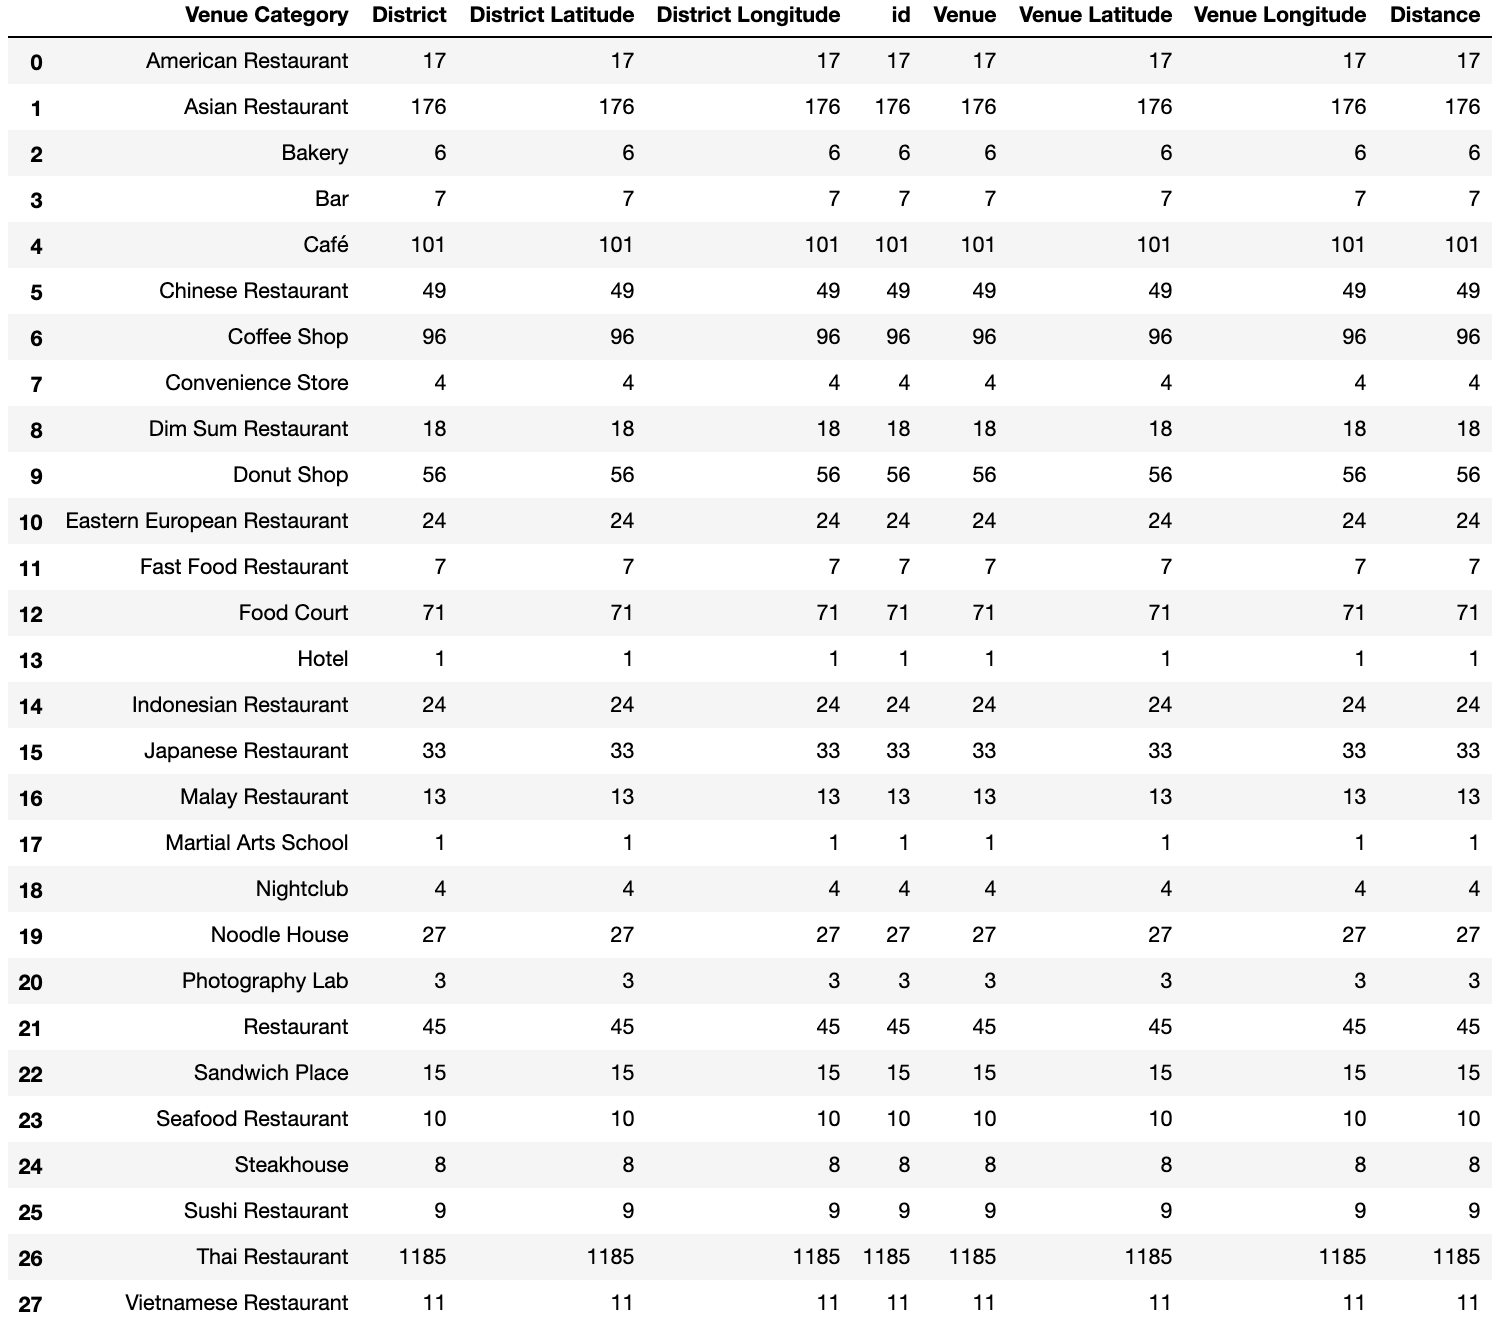
\includegraphics[width=0.7\textwidth]{fig/categories}
    \end{center}
    \caption{List of Categories}
    \label{fig:categories}
    \end{figure}
\end{center}

After cleaning the data there are only \textbf{183} Thai Restaurants. From 42 Districts, only 27 districts that have at least 1 Thai Restaurant with the highest number is 21 Thai Restaurants.

\begin{center}
    \begin{figure}[htp]
    \begin{center}
     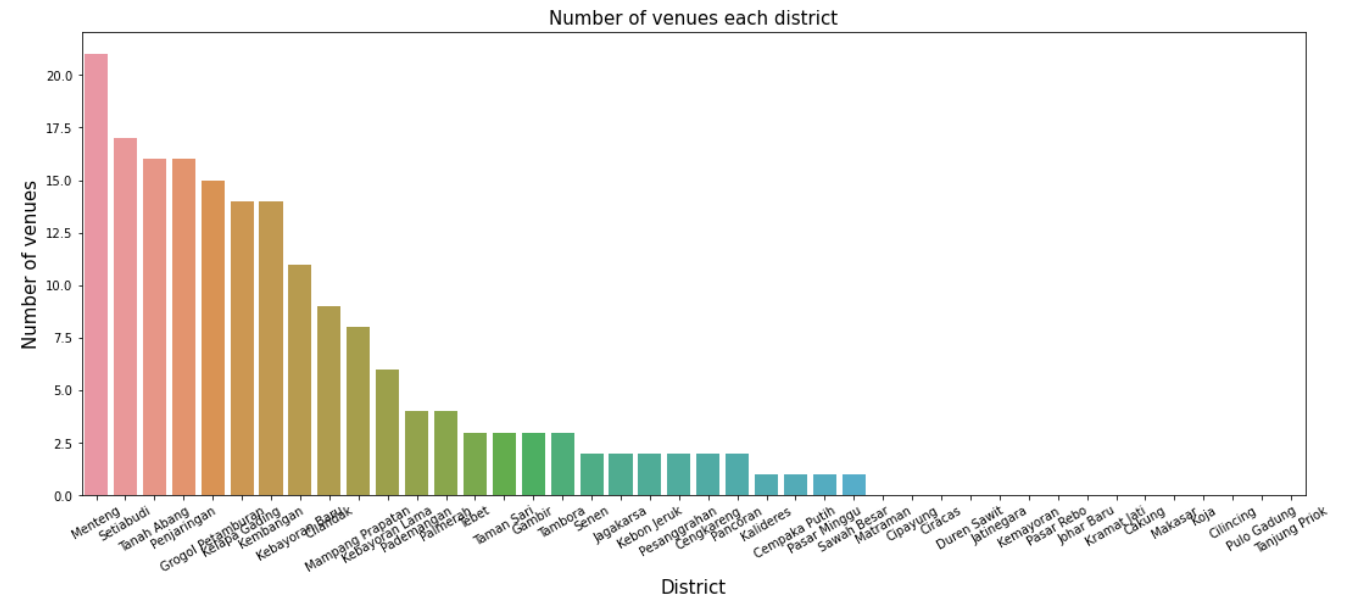
\includegraphics[width=0.8\textwidth]{fig/venue_district}
    \end{center}
    \caption{Number of Venue in District}
    \label{fig:venue_district}
    \end{figure}
\end{center}
 
\clearpage

\subsection{Clustering}

We want to cluster them into several groups based on \textbf{Average Housing Price}, \textbf{Density}, and \textbf{number of Venues}

\begin{center}
    \begin{figure}[htp]
    \begin{center}
     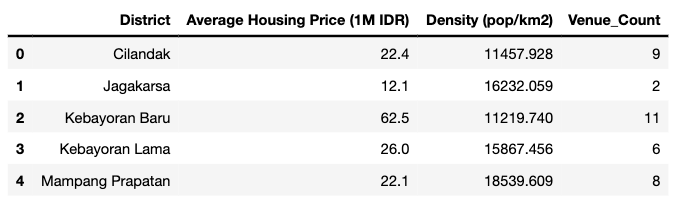
\includegraphics[width=\textwidth]{fig/cluster}
    \end{center}
    \caption{Cluster Data}
    \label{fig:cluster}
    \end{figure}
\end{center}

First, we need to determine the number of groups (or K for the K-means method). Using the elbow method with different values of K, Figure~\ref{fig:elbow} shows that \textbf{4} is the best choice.

\begin{center}
    \begin{figure}[htp]
    \begin{center}
     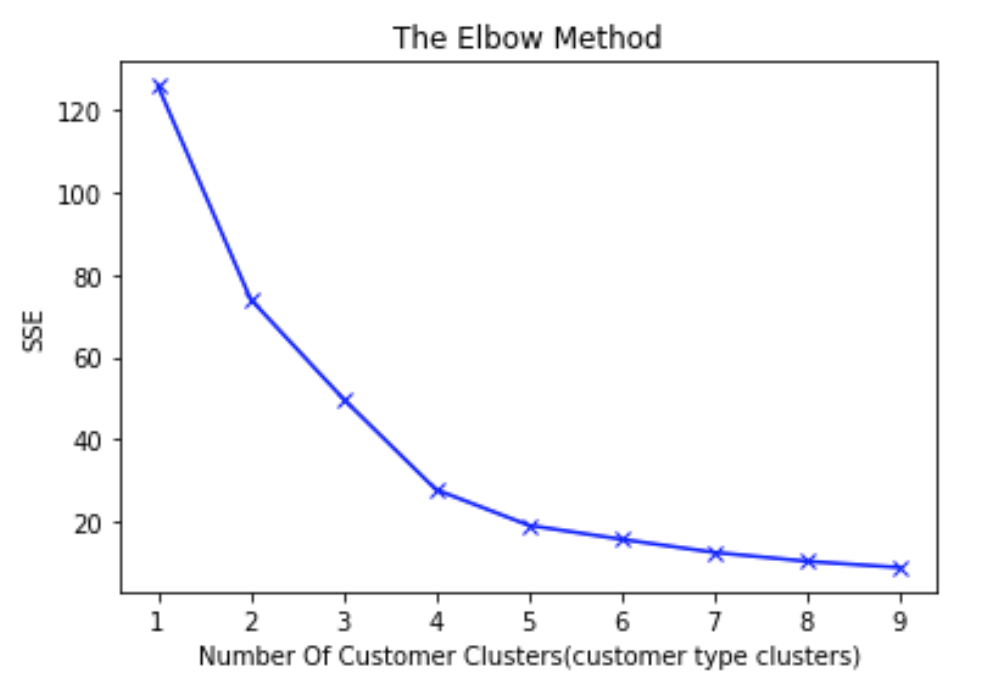
\includegraphics[width=\textwidth]{fig/elbow}
    \end{center}
    \caption{The optimal number of clusters}
    \label{fig:elbow}
    \end{figure}
\end{center}

\clearpage

\section{Results}

Here is my merged table with cluster labels for each district.

\begin{center}
    \begin{figure}[htp]
    \begin{center}
     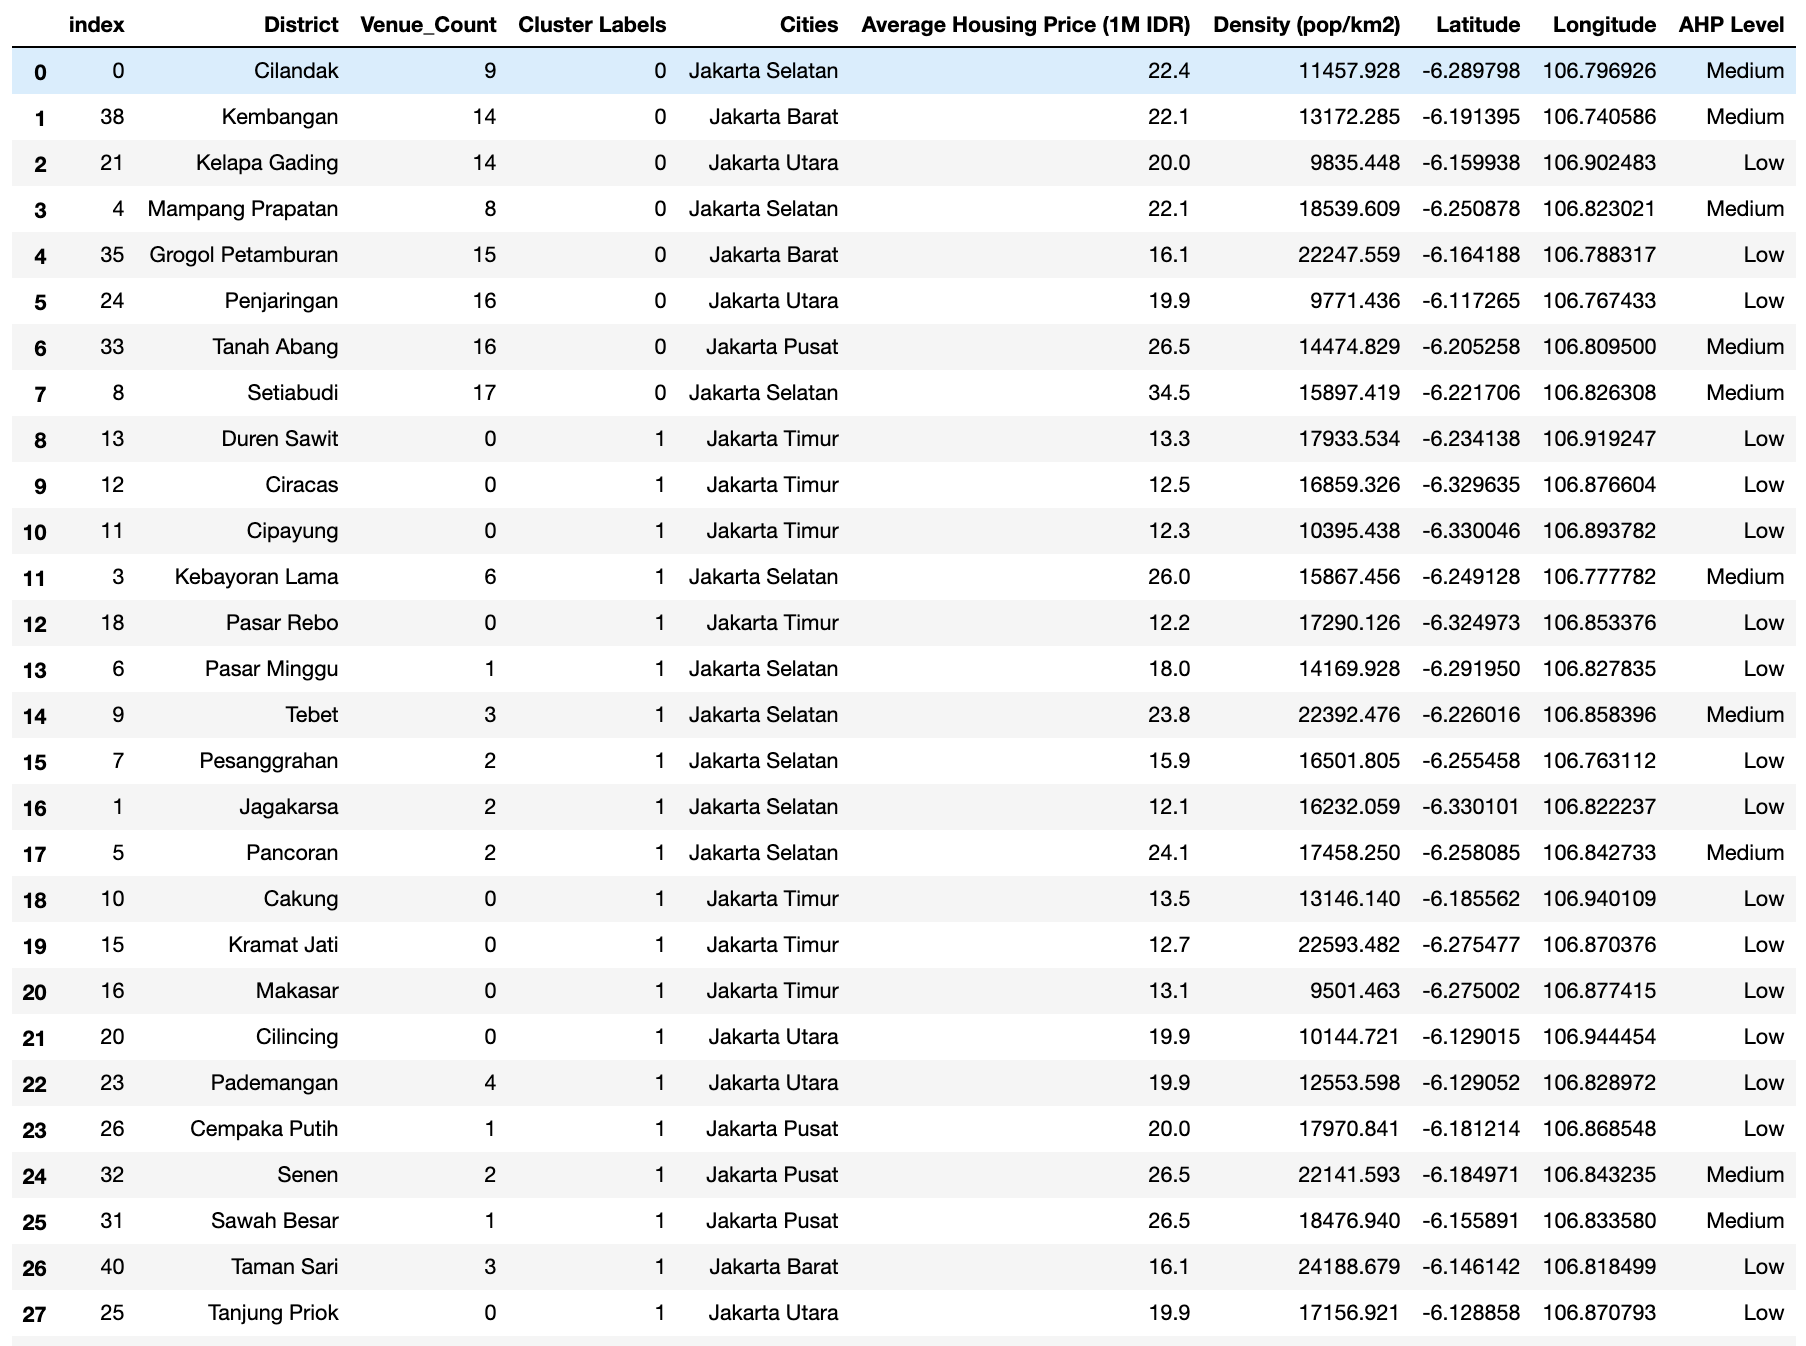
\includegraphics[width=\textwidth]{fig/cluster_label}
    \end{center}
    \caption{Merged Table with clusters}
    \label{fig:cluster_label}
    \end{figure}
\end{center}

We can label the clusters like these and put it to the main data frame:
\begin{itemize}
\item \textbf{Cluster 0} : There are a lot of Thai Restaurants in these districts, and the AHP price is medium.
\item \textbf{Cluster 1} : There are not many Thai Restaurants in these districts, and the AHP price is low.
\item \textbf{Cluster 2} : There are a lot of Thai Restaurants in these districts, and the AHP price is high.
\item \textbf{Cluster 3} : The number of Thai Restaurants in these districts are low, the AHP price is low, but the density is high
\end{itemize}

\clearpage

Figure~\ref{fig:cluster_map} illustrates the clusters of all districts in Jakarta. With this map, we can easily distinguish the clusters between districts.

\begin{center}
    \begin{figure}[htp]
    \begin{center}
     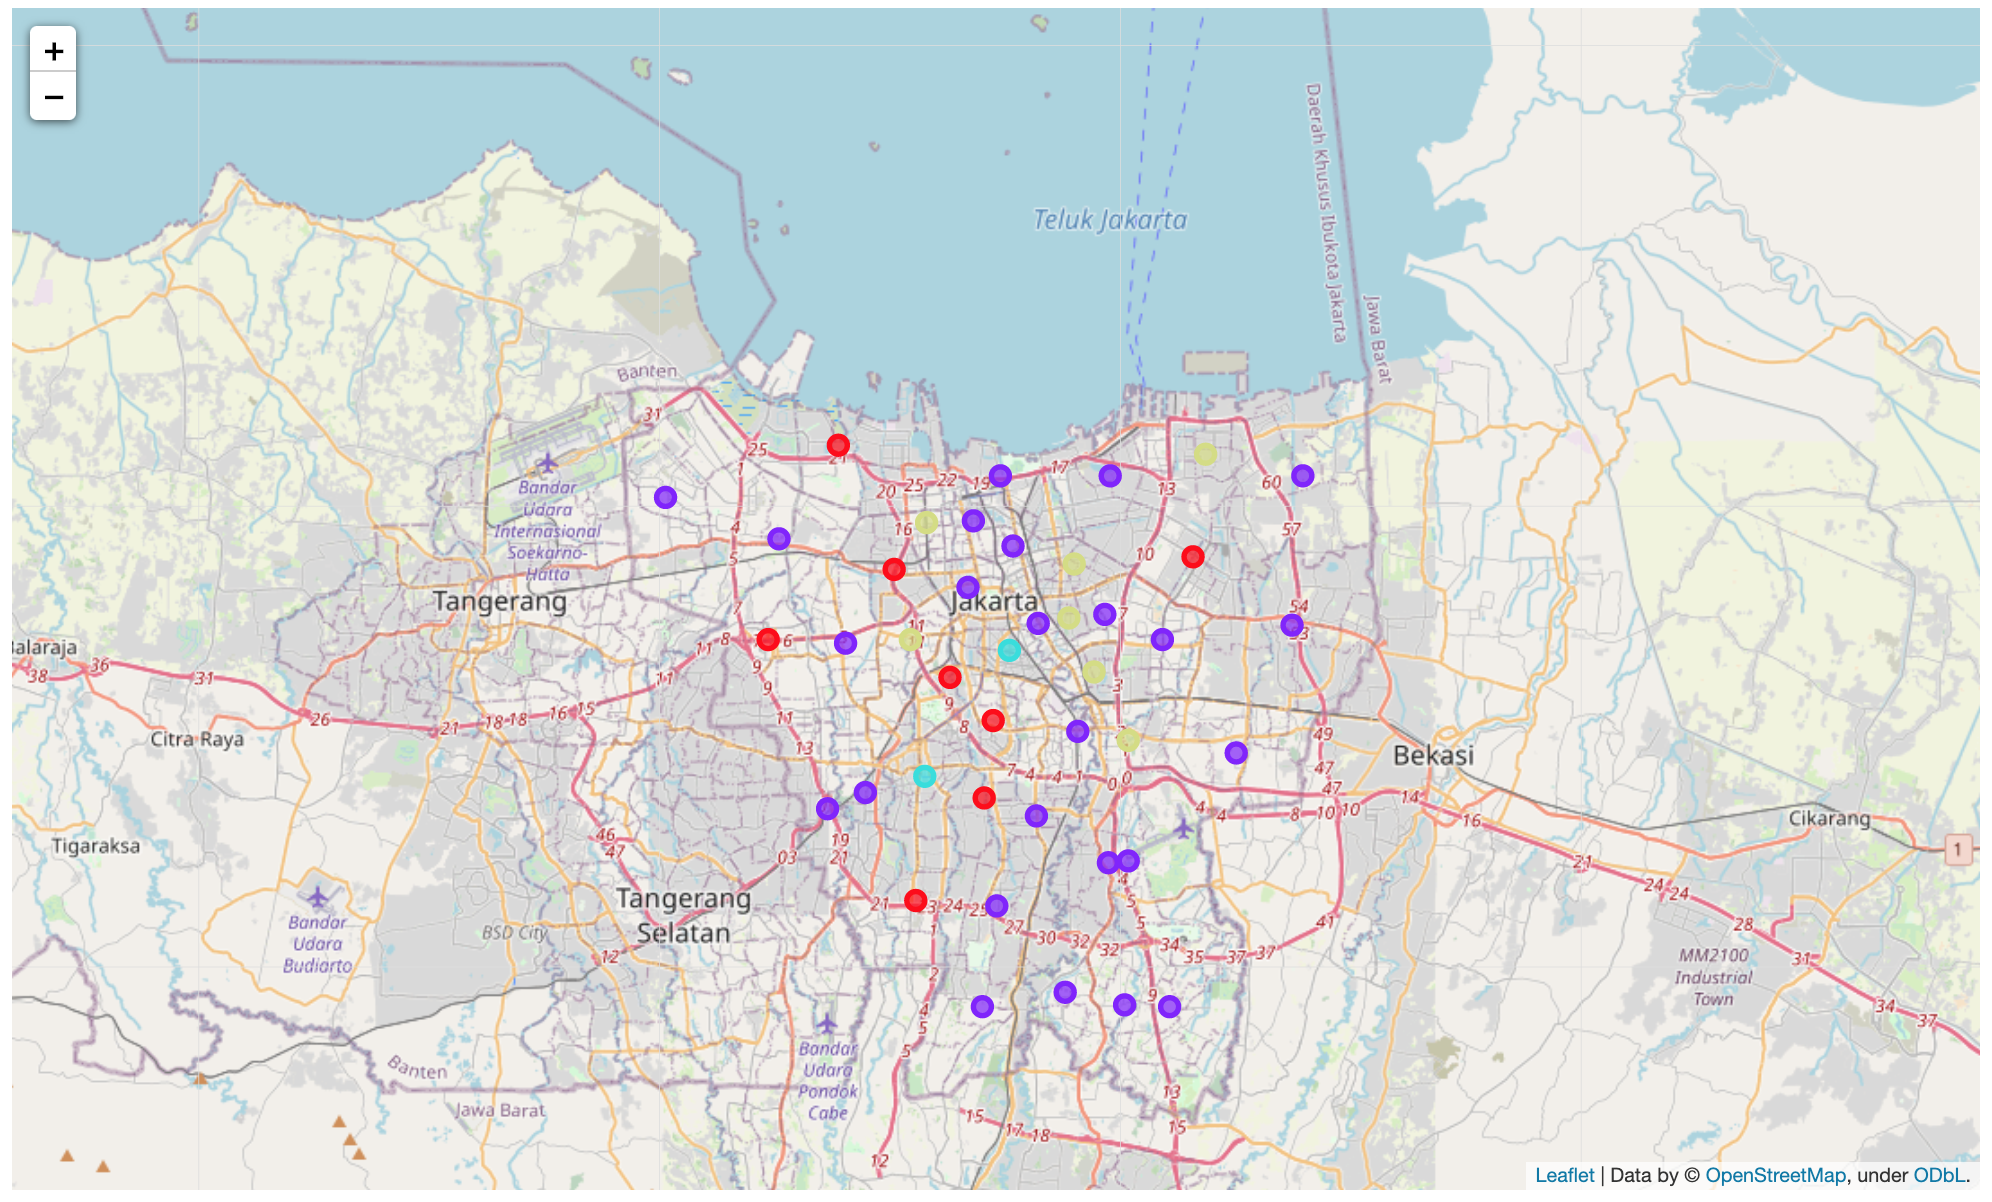
\includegraphics[width=0.8\textwidth]{fig/cluster_map}
    \end{center}
    \caption{The maps of clusters}
    \label{fig:cluster_map}
    \end{figure}
\end{center}

If we look back to the average housing price table (AHP), we can define them into 3 groups (unit: million IDR). Figure~\ref{fig:ahp} indicates that the low price housing take the majority. We need to focus on the \textbf{Low} housing price to set up our business.

\begin{itemize}
\item \textbf{Low} : $10 < AHP \le 20$.
\item \textbf{Medium} : $20 < AHP \le 50$.
\item \textbf{High} : $50 \le AHP$.
\end{itemize}

\begin{center}
    \begin{figure}[htp]
    \begin{center}
     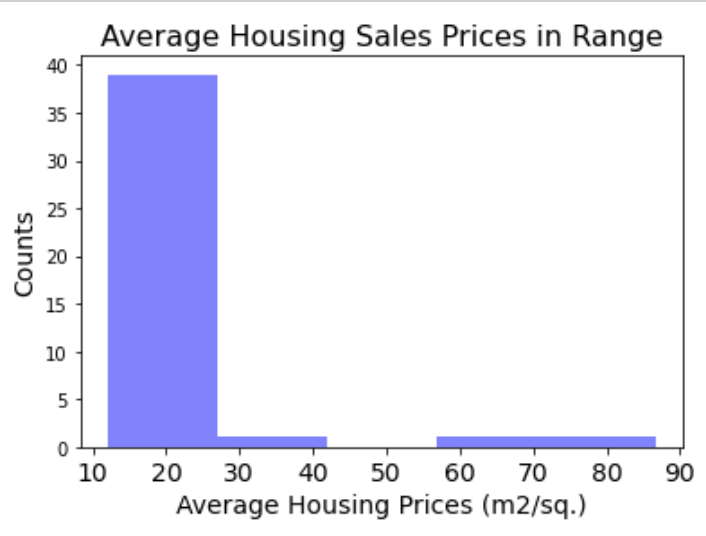
\includegraphics[width=0.5\textwidth]{fig/ahp}
    \end{center}
    \caption{The distribution of AHP.}
    \label{fig:ahp}
    \end{figure}
\end{center}

\clearpage

Figure~\ref{fig:ahp_map} shows us the choropleth map of AHP.

\begin{center}
    \begin{figure}[htp]
    \begin{center}
     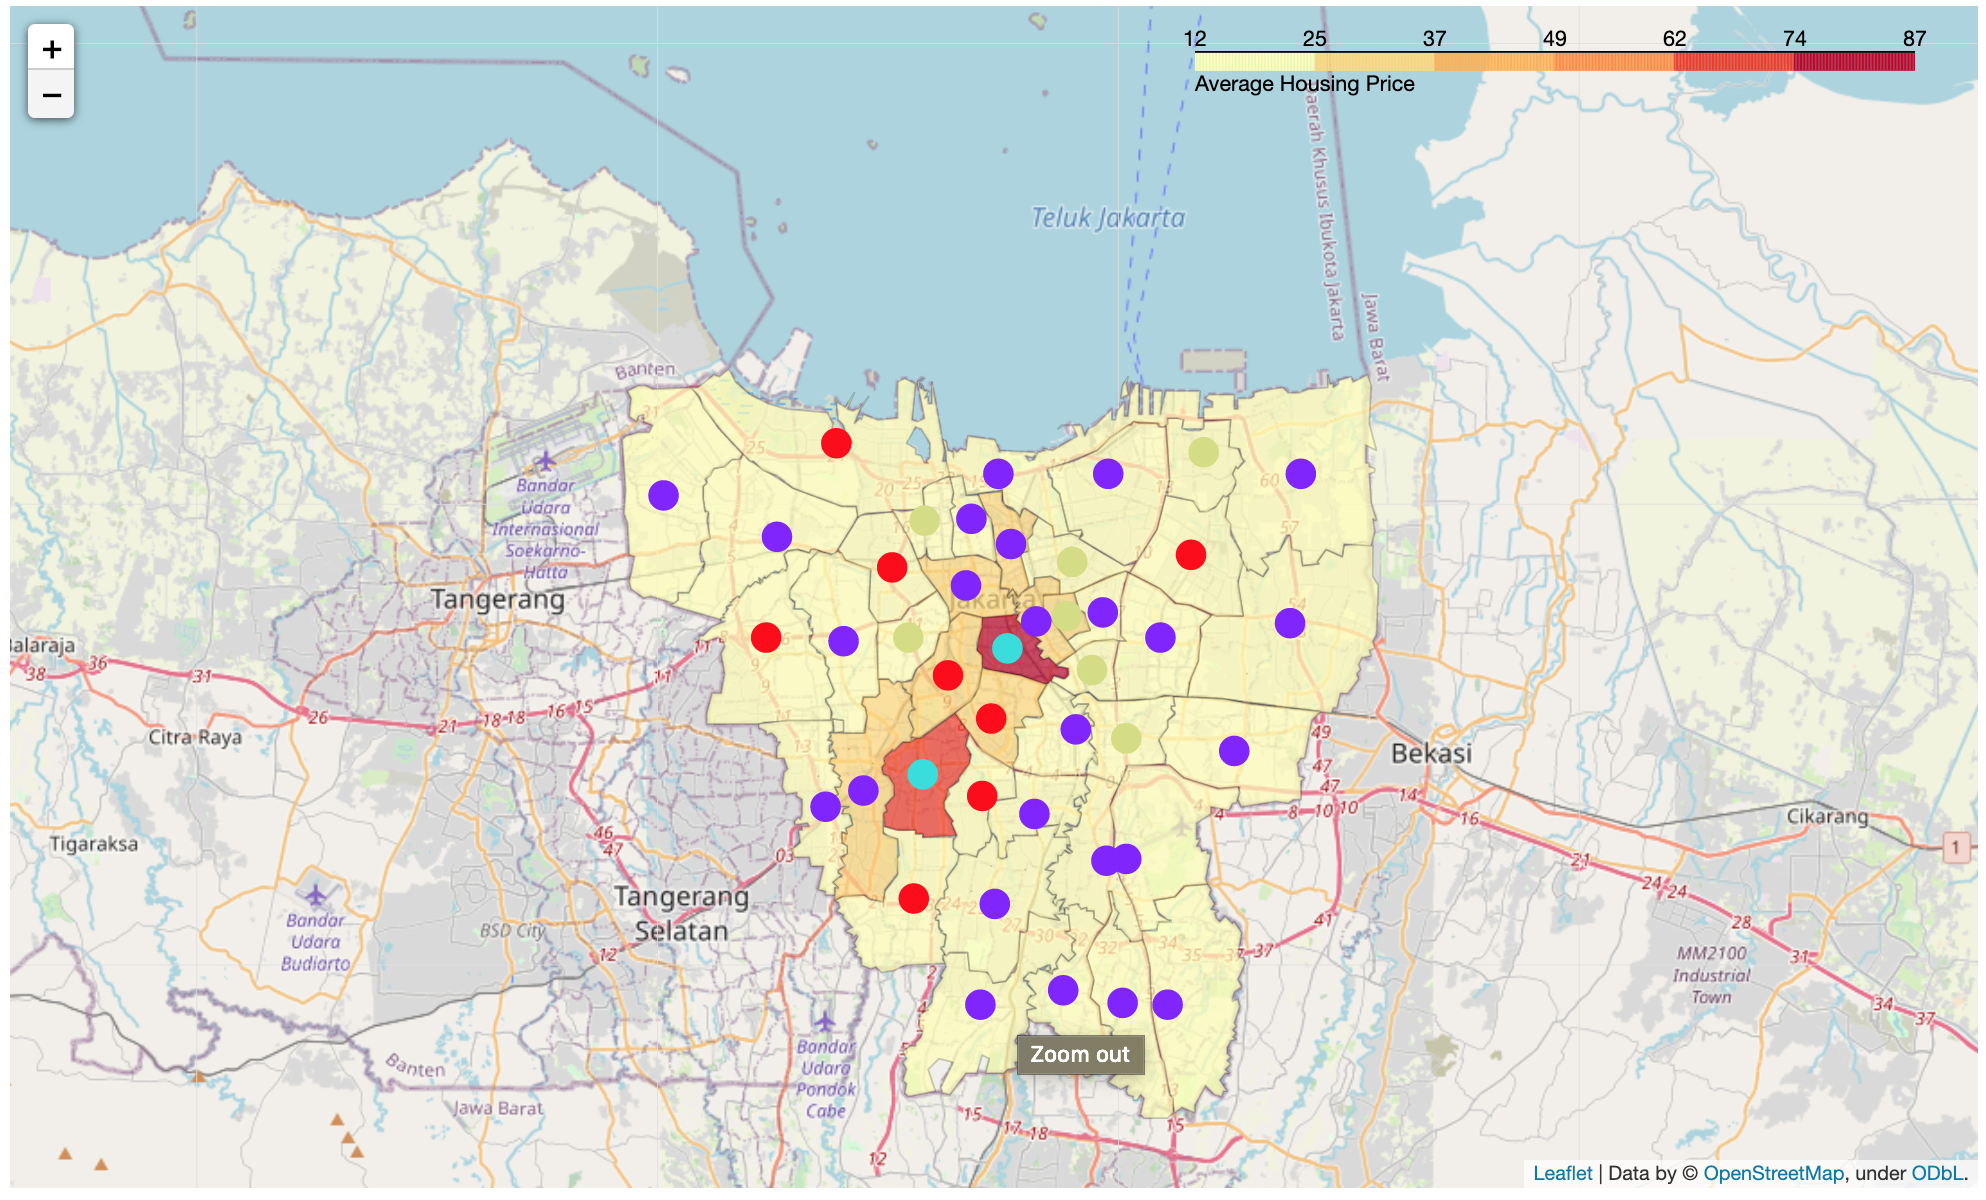
\includegraphics[width=0.8\textwidth]{fig/ahp_map}
    \end{center}
    \caption{The couple maps of AHP and the clusters}
    \label{fig:ahp_map}
    \end{figure}
\end{center}

We also can see the relationship between Density and clusters. Figure~\ref{fig:density_map} gives us a full picture about the relation between population density and the clusters.

\begin{center}
    \begin{figure}[htp]
    \begin{center}
     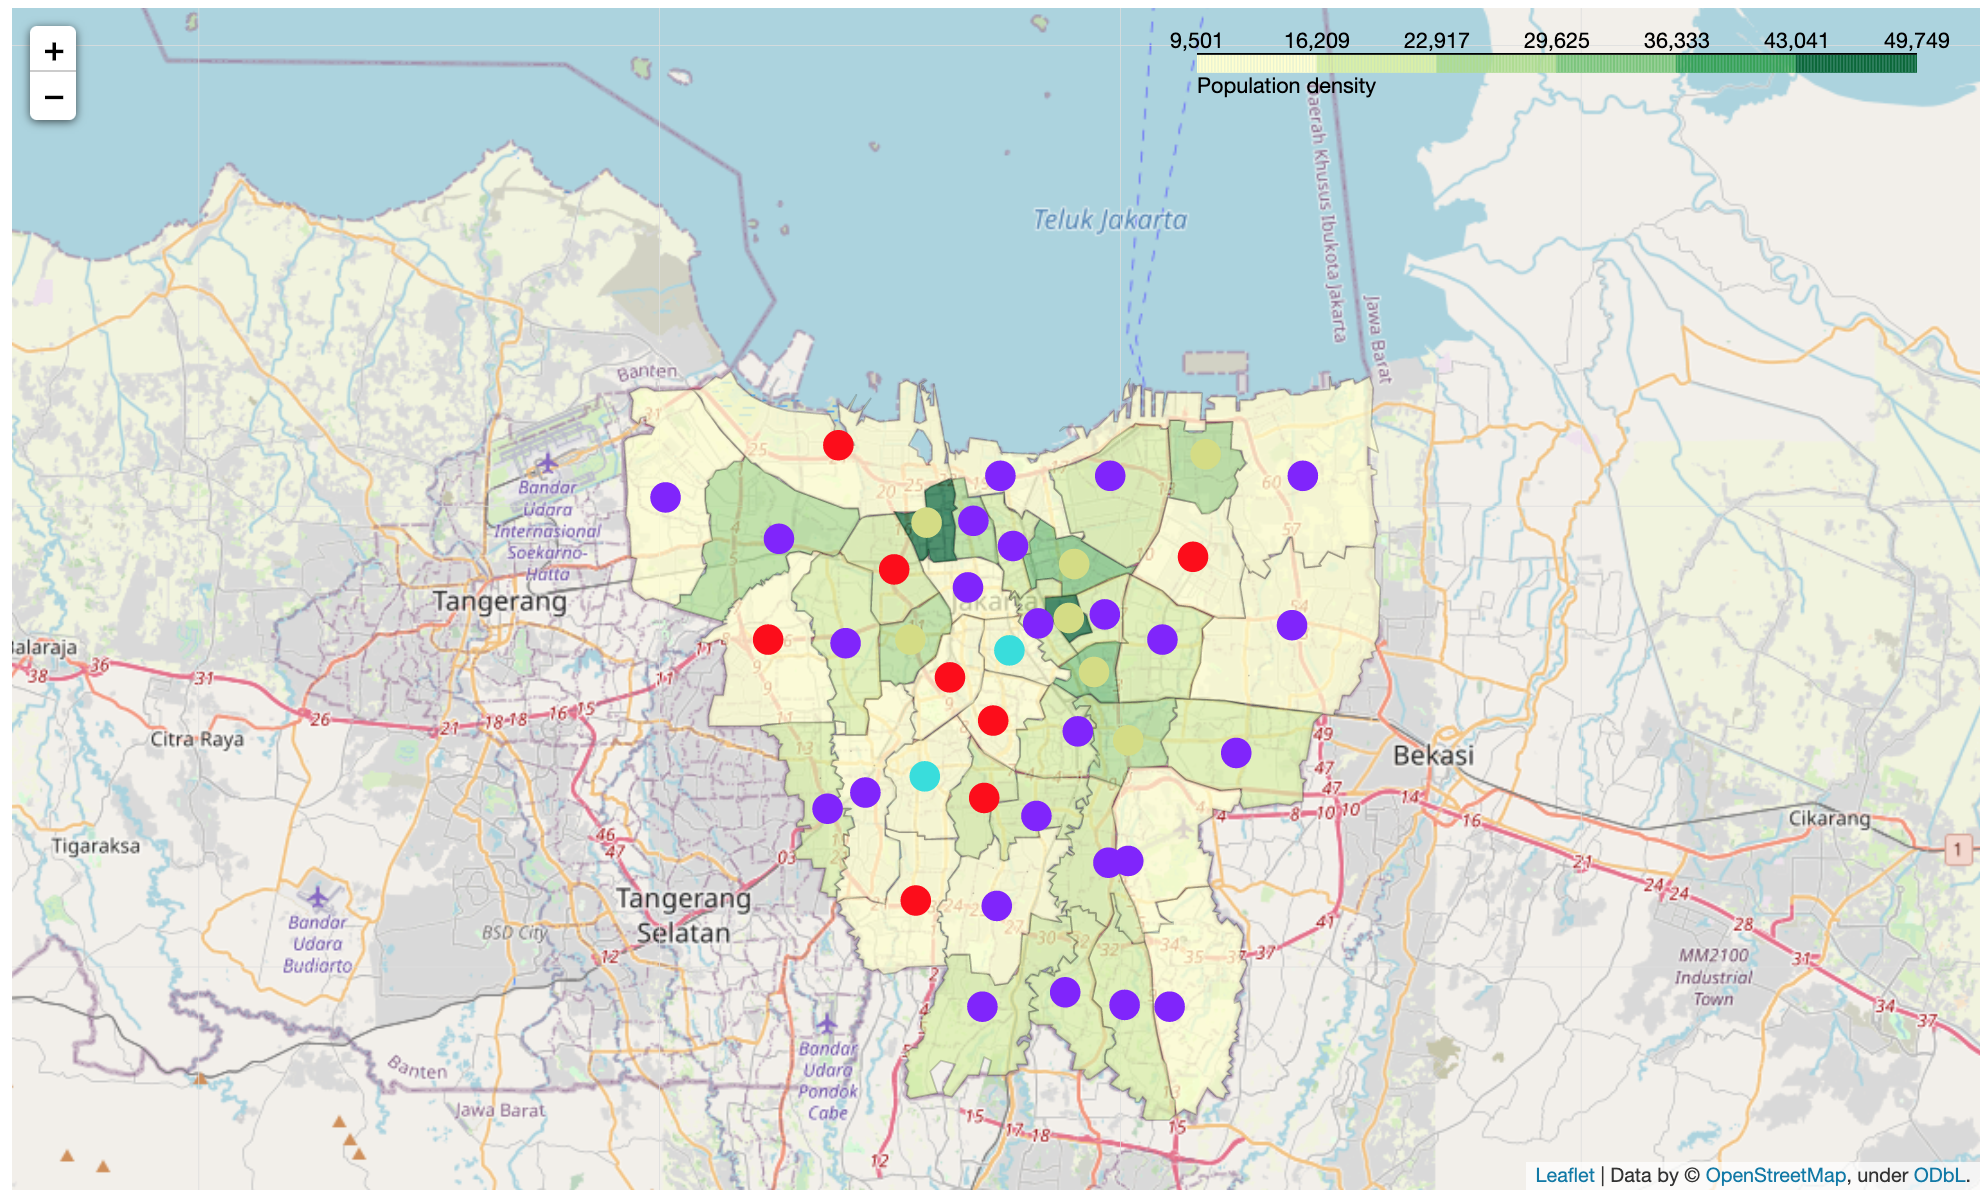
\includegraphics[width=0.8\textwidth]{fig/density_map}
    \end{center}
    \caption{The couple maps of clusters and the population density of each district.}
    \label{fig:density_map}
    \end{figure}
\end{center}

\clearpage

We focus on Cluster 3: 

\begin{itemize}
\item Where there are \textbf{not many Thai Restaurants} + \textbf{Low AHP Price} + \textbf{High density}: \textbf{Matraman}, \textbf{Jatinegara}, \textbf{Palmerah}, \textbf{Tambora}, \textbf{Kemayoran}, \textbf{Koja}, and \textbf{Johar Baru}
\end{itemize}

\begin{center}
    \begin{figure}[htp]
    \begin{center}
     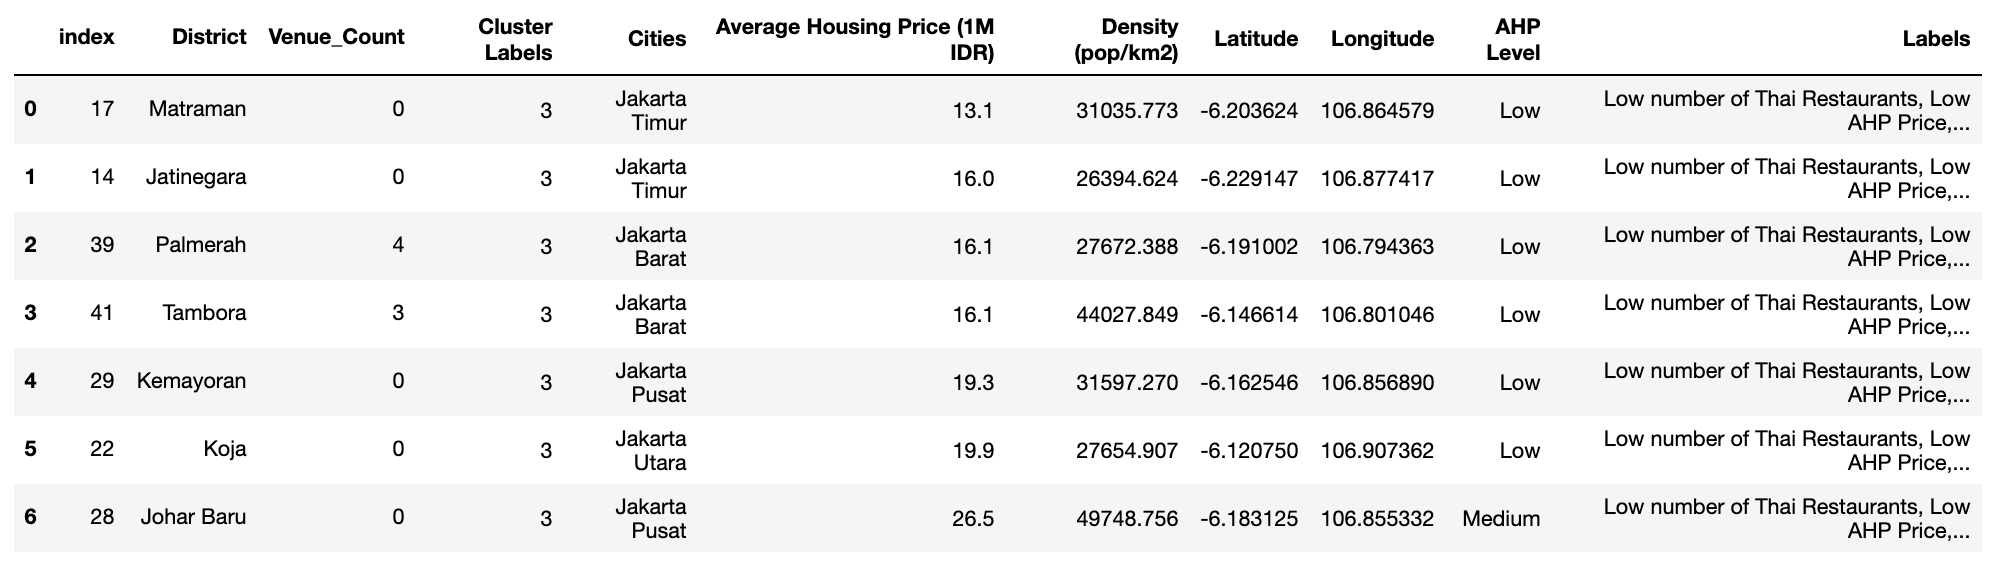
\includegraphics[width=\textwidth]{fig/result}
    \end{center}
    \caption{Cluster 3}
    \label{fig:result}
    \end{figure}
\end{center}

\section{Conclusion}

From all above results, we conclude that the best place for us to set up a new Thai Restaurant is in \textbf{cluster 3} because there are a lot of people living there (high density), there are not many already-working Thai Restaurant and the average housing price is low.

There are 7 districts in cluster 3, but if we have to choose one District, \textbf{Matraman} is the best district over cluster 3, because it has the lowest Average Housing Price and the density is high.

\end{document}
